\chapter{Overview}\label{ch:overview}
%evtl. in related work als Einleitende subsections

This chapter briefly gives an overview of the terminology in clustering and categorizes its different branches. We mention a variety of existing clustering algorithms to give a basic understanding of the different archetypes. Additionally, we give insights into correlation clustering in particular, being a vital/core branch for the sake of this work. Concrete implementations of \autoref{sec:subspaceclu} will be further elaborated in \autoref{sec:Related Work} and \autoref{ch:Methods}. For an in-depth explanation of the mentioned algorithms in \autoref{fig:clusteringtree}, we refer to its respective references.

\section{Clustering}\label{sec:clu}
% Clustering is the process of grouping a set of data objects into groups of \textit{similar} objects. 
Clustering (or Cluster Analysis) is the unsupervised process of grouping a set of data objects into classes by maximizing the similarity of the data objects within a class and minimizing the similarity across data objects of other classes. How the measure of the \textit{``similarity''} is defined, is subject to the objective of the clustering, which is dependent on the task and could demand e.g.\ a similarity in attributes or a similarity in distribution. 

Cluster Analysis proves to be advantageous in scenarios, where the data is unlabelled or too extensive to be human-processible. It can reveal unknown structures or generalize too complex patterns/structures to assist human comprehension and is considered a significant task in exploratory data mining and statistical data analysis. Due to its capabilities, clustering is used in a large variety of fields, such as physics, medicine, biology, geography, psychology, marketing etc.\ to preprocess data or reveal/augment information~\cite{kriegel2009clustering}.
As previously mentioned, the task of clustering is dependent on a \textit{similarity}-measure which is subject to an objective goal. Based on the objective and inspired by \textcite{validationhalkidi2001clustering} and \textcite[Ch.10.1.3]{han2011data} we broadly categorize the cluster analysis into four branches of clustering: Partitioning Clustering, Density-based Clustering, Hierarchical Clustering and Subspace Clustering. 
% Clustering is an unsupervised machine learning/exploratory data mining task and is the process of grouping a set of data objects into groups of \textit{similar} objects. The keyword \textit{``similar''} is dependent on the objective goal of the clustering which is dependent on the task and could demand similar attributes, e.g. finding similar data points, or similar relationships, e.g. data points following a trend. Formally one could state:
% Given data objects $o_i, i\in\{1,2,...,n\}$ with a set of attributes $a_j, j\in\{1,2,...,d\}$. Our data set $ds$ is a set of data objects $ds=\{o_1, o_2, ... , o_n\}$ with $n$ observations which respectively have $d$ Dimensions/attributes. $f$ is a function which Clustering is the optimization problem of minimizing a function $f$ which simply
% These clustering approaches are based on the \textit{locality assumption}
% \begin{figure}
%     \centering
%     \makebox[\textwidth][c]{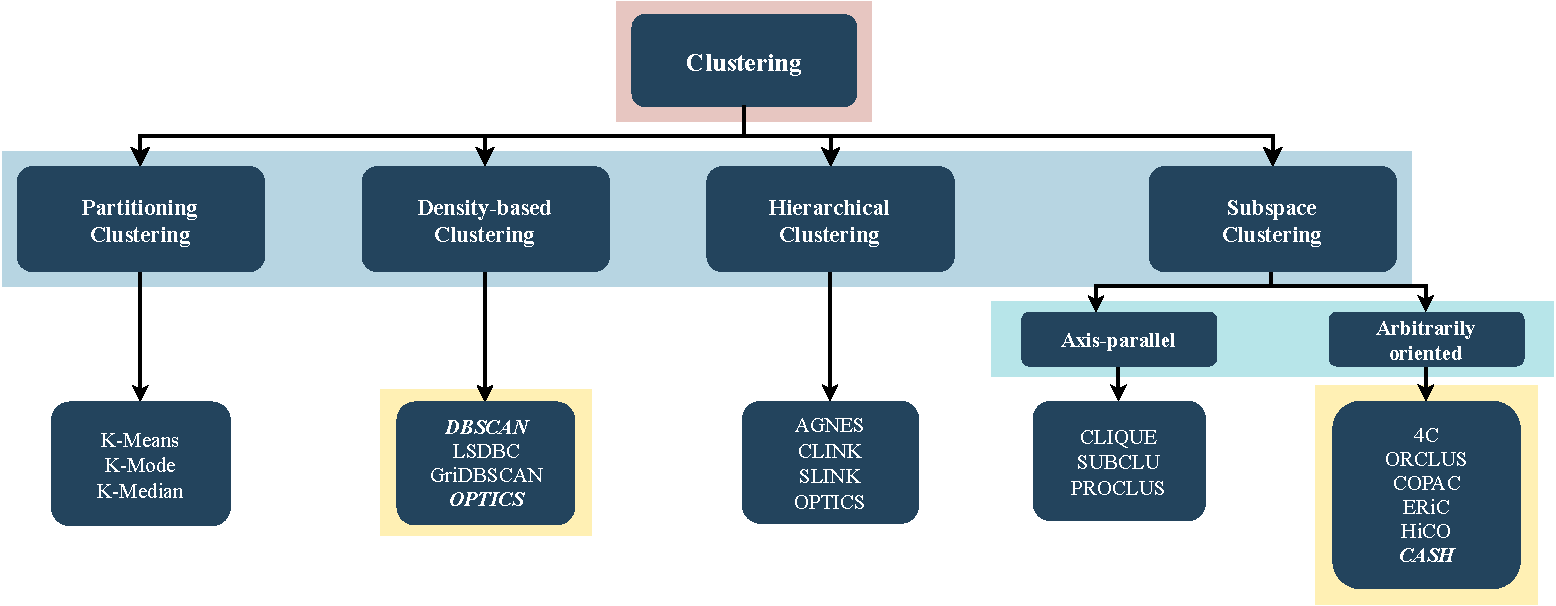
\includegraphics[width=1.1\textwidth, page=1]{figures/ClusteringAxis.pdf}}
%     \caption{Objective-oriented categorization of Clustering, Yellow marked areas are the main focus of the thesis}
%     \label{fig:clusteringtree}
% \end{figure}

\begin{figure}
    \centering
    \makebox[\textwidth][c]{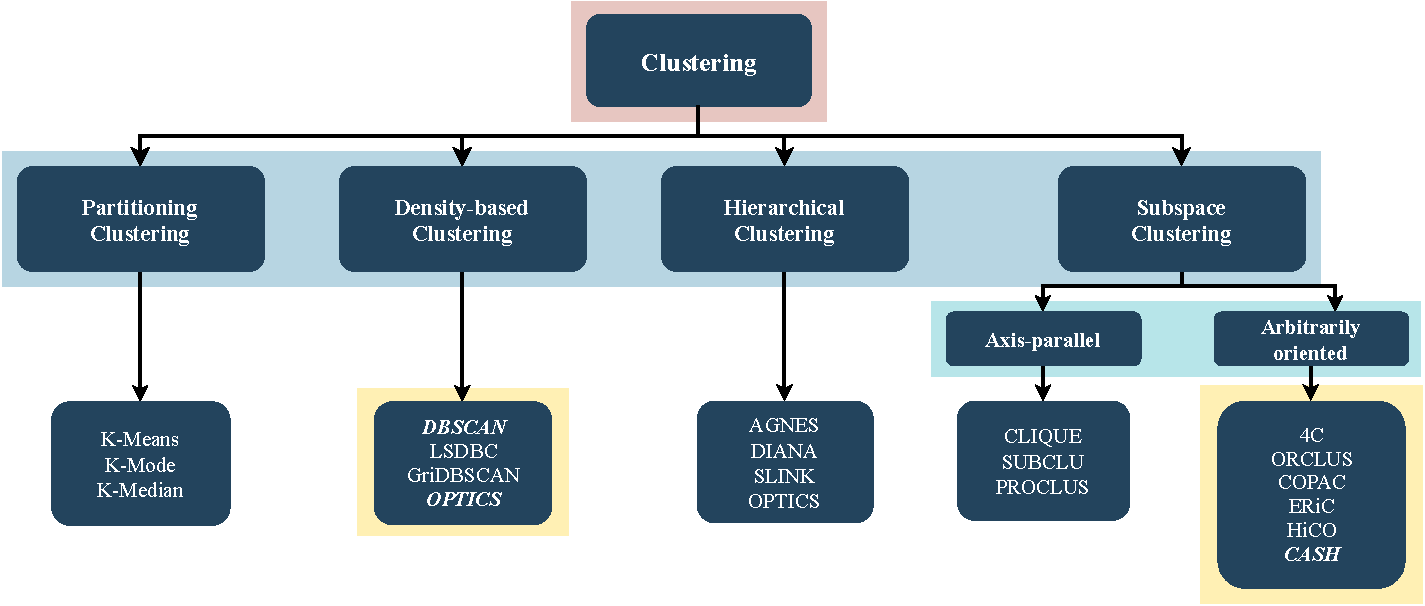
\includegraphics[width=1.1\textwidth, page=1]{figures/clusteringcatv2.pdf}}
    \caption{Objective-oriented categorization of clustering; yellow marked areas are the main focus of the thesis.}
    \label{fig:clusteringtree}
\end{figure}


% \todog{als items oder ssecs? detailliert genug? mit oder ohne formeln?}
\begin{itemize}
    \item \textbf{Partitioning Clustering:} has the objective of partitioning the whole data space into a predefined number of disjunct partitions optimizing a certain criterion function. It is one of the simplest and most fundamental versions of cluster analysis~\cite[Ch.10.2]{han2011data}.
    % \todor{citation mit gemischtem style? ist das erste buch, ohne seitennummer findet man das ja nie; DK: nur das Buch wie sonst bei den Papern auch zitieren und in Klammern dahinter so etwas wie z.B. (Ch.10.2), bzw. auch in der Klammer.}
    % has the objective of partitioning the whole data space $DS$ into $k, k \in \N$ disjunct partitions $P_i, i \in \{1,\dotsc,k\}$ with $\bigcup^k_{j=1} P_j = DS$, optimizing a certain criterion function.
    
    Common implementations of this archetype of clustering are \linebreak $k$-Means~\cite{kmeansmacqueen1967some} and its derivations, e.g. $k$-Modes and $k$-Medians~\cite{kmeanshalfcenturysteinley2006k}. They cluster the data space into $k$ partitions, minimizing the criterion of the squared error to the partitions' respective means/modes/medians and tend to build clusters in convex shapes~\cite{clusteringsurveyberkhin2006survey}. 
    % \todor{L: welchen begriff benutzen, /excel at building/}
    
    Partitioning clustering algorithms like $k$-Means often are used due to their ease of implementation, simplicity, efficiency, and empirical success~\cite{kmeans50jain2010data}.
    However, these types of partitioning algorithms come with a few disadvantages. It is hard to determine a sensible $k$ and the clustering is sensitive to noise and outliers~\cite{dataclusteringreviewjain1999data}. 
    
    \item \textbf{Density-based Clustering:} attempts to group neighbouring objects $o$ in a data space $DS$ into clusters based on a density condition and separates them by sparse regions of low density. In contrast to partitioning clustering, density-based clustering is not as sensitive to noise and outliers. Additionally, it is not restricted to just finding convex partitions, but also arbitrarily shaped clusters~\cite[Ch.10.4]{han2011data}.
    
    A well-known implementation of this archetype of clustering is \acrshort{dbscan}~\cite{DBSCANEKSX96}. Its general idea is to continue growing a given cluster as long as the density in a certain neighbourhood exceeds a certain threshold. 
    
    \item \textbf{Hierarchical Clustering:} Unlike partitioning and density-based clustering, \textit{Hierarchical clustering} is not just segmenting the data space once but intends to create a hierarchical decomposition of a given set of data objects. This hierarchy can be for example constructed by starting with the whole data space as one cluster and iteratively splitting it into smaller clusters while keeping relationships to its parents, or by considering each data object as a cluster first and iteratively merging those into bigger clusters. The first variant is called a \textit{top-down} approach, also known as \textit{divisive}, and the second variant is called \textit{bottom-up} approach, also known as \textit{agglomerative}~\cite[Ch.10.3]{han2011data}. 
    
    An instance of a divisive algorithm is \acrshort{diana}~\cite[Ch.6]{kaufman2009finding}, and an agglomerative example is \acrshort{agnes}~\cite[Ch.5]{kaufman2009finding}.
    
    
    \item \textbf{Subspace Clustering:} The defining feature of previously mentioned archetypes is the clustering based on a full-dimensional spatial structure like partitioning, density or hierarchy. \textit{Subspace clustering} can be used in conjunction with the other archetypes since it has the primary goal of finding the relevant \textit{subspaces} of clusters in the original data space. This is especially required for high-dimensional data, since there may be many attributes irrelevant for clustering~\cite{vidal2011subspace}. 
    % \textit{Subspace clustering} has the main objective of finding relevant \textit{subspaces} of clusters of the original data space. This is especially required for high dimensional data, since there may be clusters defined by only a subset of attributes~\cite{vidal2011subspace}. 
    % since it has the primary goal of \textit{finding clusters in subspaces} or \textit{finding the relevant subspaces of clusters}
    
    Subspace clustering algorithms can be divided into two categories: Finding \textit{axis-parallel} subspaces (e.g. projected clustering) and finding \textit{arbitrarily oriented} subspaces (e.g.\ correlation clustering)~\cite[Ch.3]{zimek2009correlation}.
    For completeness, \textcite{zimek2009correlation} also defines a third category, called pattern-based clustering, which looks at patterns in the data matrix, a matrix representing the data space. This clustering, however, does not have a spatial interpretation and is therefore omitted in our categorization.
    
    % \todor{L: Wie zitier ich das, wenn ich nur zu 66\% zustimme? :D Ich stimme einfach nicht mit der terminology zu. MMn sollte es nur axis-parallel(projected) und arbitrary oriented(correlation) geben, patternbased clustering zaehlt fuer mich nicht zu subspace clustering.}
    
    Axis-parallel methods include \acrshort{clique}~\cite{cliqueagrawal1998automatic}, \acrshort{proclus}~\cite{proclusaggarwal1999fast}, etc., and arbitrarily oriented implementations include \acrshort{4c}~\cite{4cbohm2004computing}, \acrshort{orclus}~\cite{orclusaggarwal2000finding}, \acrshort{cash}~\cite{CASHachtert2008global}, etc.
\end{itemize}

% % Please add the following required packages to your document preamble:
% % \usepackage{booktabs}
% % \usepackage{graphicx}
% \begin{table}[]
% \centering
% \resizebox{\textwidth}{!}{%
% \begin{tabular}{@{}|l|l|@{}}
% \toprule
% \textbf{Method}                   & \textbf{General Characteristics}                                                                                                                                                                                                                                                                                    \\ \midrule
% Partitioning Clustering  & \begin{tabular}[c]{@{}l@{}}\tabitem Find mutually exclusive clusters of convex shape\\ \tabitem Distance-based\\ \tabitem May use mean or medoid (etc.) to represent cluster center\\ \tabitem Effective for small- to medium-size data sets\end{tabular}                                                                           \\ \midrule
% Density-based Clustering & \begin{tabular}[c]{@{}l@{}}\tabitem Can find arbitrarily shaped clusters\\ \tabitem Clusters are dense regions of objects in space that are separated \\ \quad \ by low-density regions\\ \tabitem Cluster density: Each point must have a minimum number of\\ \quad \  points within its neighborhood\\ \tabitem May filter out noise and outliers\end{tabular} \\ \midrule
% Hierarchical Clustering  & \begin{tabular}[c]{@{}l@{}}\tabitem Clustering is a hierarchical decomposition\\ \tabitem Cannot correct erroneous merges or splits\\ \tabitem May incorporate other techniques like microclustering or\\ \quad \ consider object ``linkages''\end{tabular}                                                       \\ \midrule
% Subspace Clustering      & \begin{tabular}[c]{@{}l@{}} \tabitem Find clusters in relevant subspaces\\ \tabitem Find relevant subspaces and correlations\\ \tabitem Subspaces/correlations can be modeled as hyperplanes\\ \tabitem Subspace/Correlation clusters are points in a neighborhood\\ \quad \ close to a hyperplane \end{tabular}                                                                                                                                                                                 \\ \bottomrule
% \end{tabular}%
% }
% \caption{Overview of clustering methods based on objective. Note that some algorithms may
% combine various methods. Adapted from ~\cite[Ch.10.1.3]{han2011data}.}
% \label{tab:clusteringcharacteristics}
% \end{table}
% \todor{Check Table with DK}

% Please add the following required packages to your document preamble:
% \usepackage{booktabs}
% \usepackage{graphicx}
\begin{table}[]
\centering
\resizebox{\textwidth}{!}{%
\begin{tabular}{@{}|l|l|l|@{}}
\toprule
\textbf{Method}                   & \textbf{General Characteristics}                                                                                                                                                                                                                                                                                    & \textbf{Implementations}                                                                                                                                       \\ \midrule
Partitioning Clustering  & \begin{tabular}[c]{@{}l@{}}\tabitem Find mutually exclusive clusters of spherical shape\\ \tabitem Distance-based\\ \tabitem May use mean or medoid (etc.) to represent cluster center\\ \tabitem Effective for small- to medium-size data sets\end{tabular}                                                                           & \begin{tabular}[c]{@{}l@{}}k-Means~\cite{kmeansmacqueen1967some}\\ k-Modes~\cite{kmodehuang1998extensions}\\ k-Medoids~\cite{kaufman2009finding}\end{tabular}                                                                                   \\ \midrule
Density-based Clustering & \begin{tabular}[c]{@{}l@{}}\tabitem Can find arbitrarily shaped clusters\\ \tabitem Clusters are dense regions of objects in space that are\\\quad\  separated by low-density regions\\ \tabitem Cluster density: Each point must have a minimum number of\\\quad\  points within its “neighborhood”\\ \tabitem May filter out outliers\end{tabular} & \begin{tabular}[c]{@{}l@{}}DBSCAN~\cite{DBSCANEKSX96}\\ LSDBC~\cite{biccici2007locally}\\ GriDBSCAN~\cite{uncu2006gridbscan}\\ OPTICS~\cite{opticsankerst1999optics}\end{tabular}                                                                           \\ \midrule
Hierarchical Clustering  & \begin{tabular}[c]{@{}l@{}}\tabitem Clustering is a hierarchical decomposition (i.e., multiple levels)\\ \tabitem Cannot correct erroneous merges or splits\\ \tabitem May incorporate other techniques like microclustering or\\\quad\  consider object ``linkages''\end{tabular}                                                       & \begin{tabular}[c]{@{}l@{}}AGNES~\cite[Ch.5]{kaufman2009finding}\\ DIANA~\cite[Ch.6]{kaufman2009finding}\\ SLINK~\cite{sibson1973slink}\\ OPTICS~\cite{opticsankerst1999optics}\end{tabular}                                                                                \\ \midrule
Subspace Clustering      & \begin{tabular}[c]{@{}l@{}}\tabitem Find relevant subspaces and correlations\\ \tabitem Find clusters in relevant subspaces\\ \tabitem Subspaces/correlations can be modelled as hyperplanes\\ \tabitem Subspace/correlation clusters are points in a neighborhood\\ \quad\  close to a hyperplane \end{tabular}                                                                                                                                                                                 & \begin{tabular}[c]{@{}l@{}}Axis-parallel:\\ \quad CLIQUE~\cite{cliqueagrawal1998automatic}\\ \quad SUBCLU~\cite{sublcukailing2004density}\\ \quad PROCLUS~\cite{proclusaggarwal1999fast}\\ Arbitrarily oriented:\\ \quad 4C~\cite{4cbohm2004computing}\\ \quad ORCLUS~\cite{orclusaggarwal2000finding}\\ \quad COPAC~\cite{copacachtert2007robust}\\ \quad ERiC~\cite{ericachtert2007exploring}\\ \quad HiCO~\cite{hicoachtert2006mining}\\ \quad CASH~\cite{CASHachtert2008global}\end{tabular} \\ \bottomrule
\end{tabular}%
}
\caption{Overview of clustering methods discussed in this chapter. Note that some algorithms may
combine various archetypes. Adapted from ~\cite[Ch.10.1.3]{han2011data}.}
\label{tab:clusteringcharacteristics}
\end{table}
% Partitional clustering attempts to directly decompose the data set into a set of disjoint
% clusters. More specifically, they attempt to determine an integer number of partitions that
% optimise a certain criterion function. The criterion function may emphasize the local or
% global structure of the data and its optimization is an iterative procedure.
% • Hierarchical clustering proceeds successively by either merging smaller clusters into
% larger ones, or by splitting larger clusters. The result of the algorithm is a tree of clusters,
% called dendrogram, which shows how the clusters are related. By cutting the dendrogram
% at a desired level, a clustering of the data items into disjoint groups is obtained.
% • Density-based clustering. The key idea of this type of clustering is to group neighbouring
% objects of a data set into clusters based on density conditions.
% • Grid-based clustering. This type of algorithms is mainly proposed for spatial data mining.
% Their main characteristic is that they quantise the space into a finite number of cells and
% then they do all operations on the quantised space.
% ~\cite{validationhalkidi2001clustering} 
% ~\cite{clusteringsurveyberkhin2006survey} ~\cite{dataclusteringreviewjain1999data} ~\cite{xu2005survey eher no}
% tst\\

\autoref{fig:clusteringtree} and \autoref{tab:clusteringcharacteristics} illustrate the dependencies and characteristics between the different branches and additionally provide a small overview of relevant implementations. Note that the archetypes of clustering are not decisive and the classification of the implementations is not clear-cut, as can be seen by \acrshort{optics} being a density-based and hierarchical algorithm. 

% source für 'basic verfahren' http://myweb.sabanciuniv.edu/rdehkharghani/files/2016/02/The-Morgan-Kaufmann-Series-in-Data-Management-Systems-Jiawei-Han-Micheline-Kamber-Jian-Pei-Data-Mining.-Concepts-and-Techniques-3rd-Edition-Morgan-Kaufmann-2011.pdf 
% source für subspace clustering verfahren: https://onlinelibrary-wiley-com.emedien.ub.uni-muenchen.de/doi/abs/10.1002/widm.1057
% lmu bookmarklet: https://www.ub.uni-muenchen.de/ausleihe-online/e-medien-login/index.html

% \section{The locality assumption}
\break
\section{Correlation Clustering}\label{sec:subspaceclu}

% This thesis focuses on the task of detecting global arbitrarily oriented subspaces by combining locally dense correlation clusters together. 
% \todor{Like mentioned in \autoref{sec:clu}}
\textit{Correlation clustering}, also known as oriented clustering or generalized subspace/projected clustering, in the field of data mining, is a special case of the general subspace clustering. In contrast to projected clustering, which finds subspaces based on the assumption that they are only axis-parallel, correlation clustering detects even \textit{arbitrarily oriented} subspaces in a data space. Correlation clustering can, therefore, be considered a more powerful clustering tool, but is, due to the infinite possible subspaces, a much more complex procedure than projected clustering. \autoref{fig:corrclusex}, however, shows an artificial example of a scenario where conventional projected clustering cannot give a good result and find all relevant subspaces. Except for cluster 3, which can actually be accurately clustered in an axis-parallel subspace, cluster 1 and cluster 2 are arbitrarily oriented and are modelled by a correlation of their features instead. This falls into the use case of correlation clustering. We will discuss some of the existing algorithms in \autoref{sec:Related Work}.
% \todor{einfach nicht gut. soll ich wirklich ein kapitel dazu machen?}

% One could ask, ``why bother with finding an arbitrarily oriented subspace when the axis-parallel subspace already contains given clusters''. The answer to that question can be illustrated by considering \autoref{fig:corrclusex}

Following in this thesis, \textit{subspaces} and \textit{subspace clusters}, unless explicitly stated, always refer to \textit{linear} arbitrarily oriented subspaces/correlations and their clusters. We also use \textit{correlation clustering} and \textit{subspace clustering} interchangeably.
% \gls{optics} \gls{elki} \gls{dbscan} \gls{orclus} \gls{lmclus} \gls{4c} \gls{eric} \gls{hico} \gls{cash} \gls{dmasc} \gls{ari} \gls{nmi} \gls{hnf} \gls{subclu} \gls{clique} \gls{pca}
\begin{figure}
    \centering
    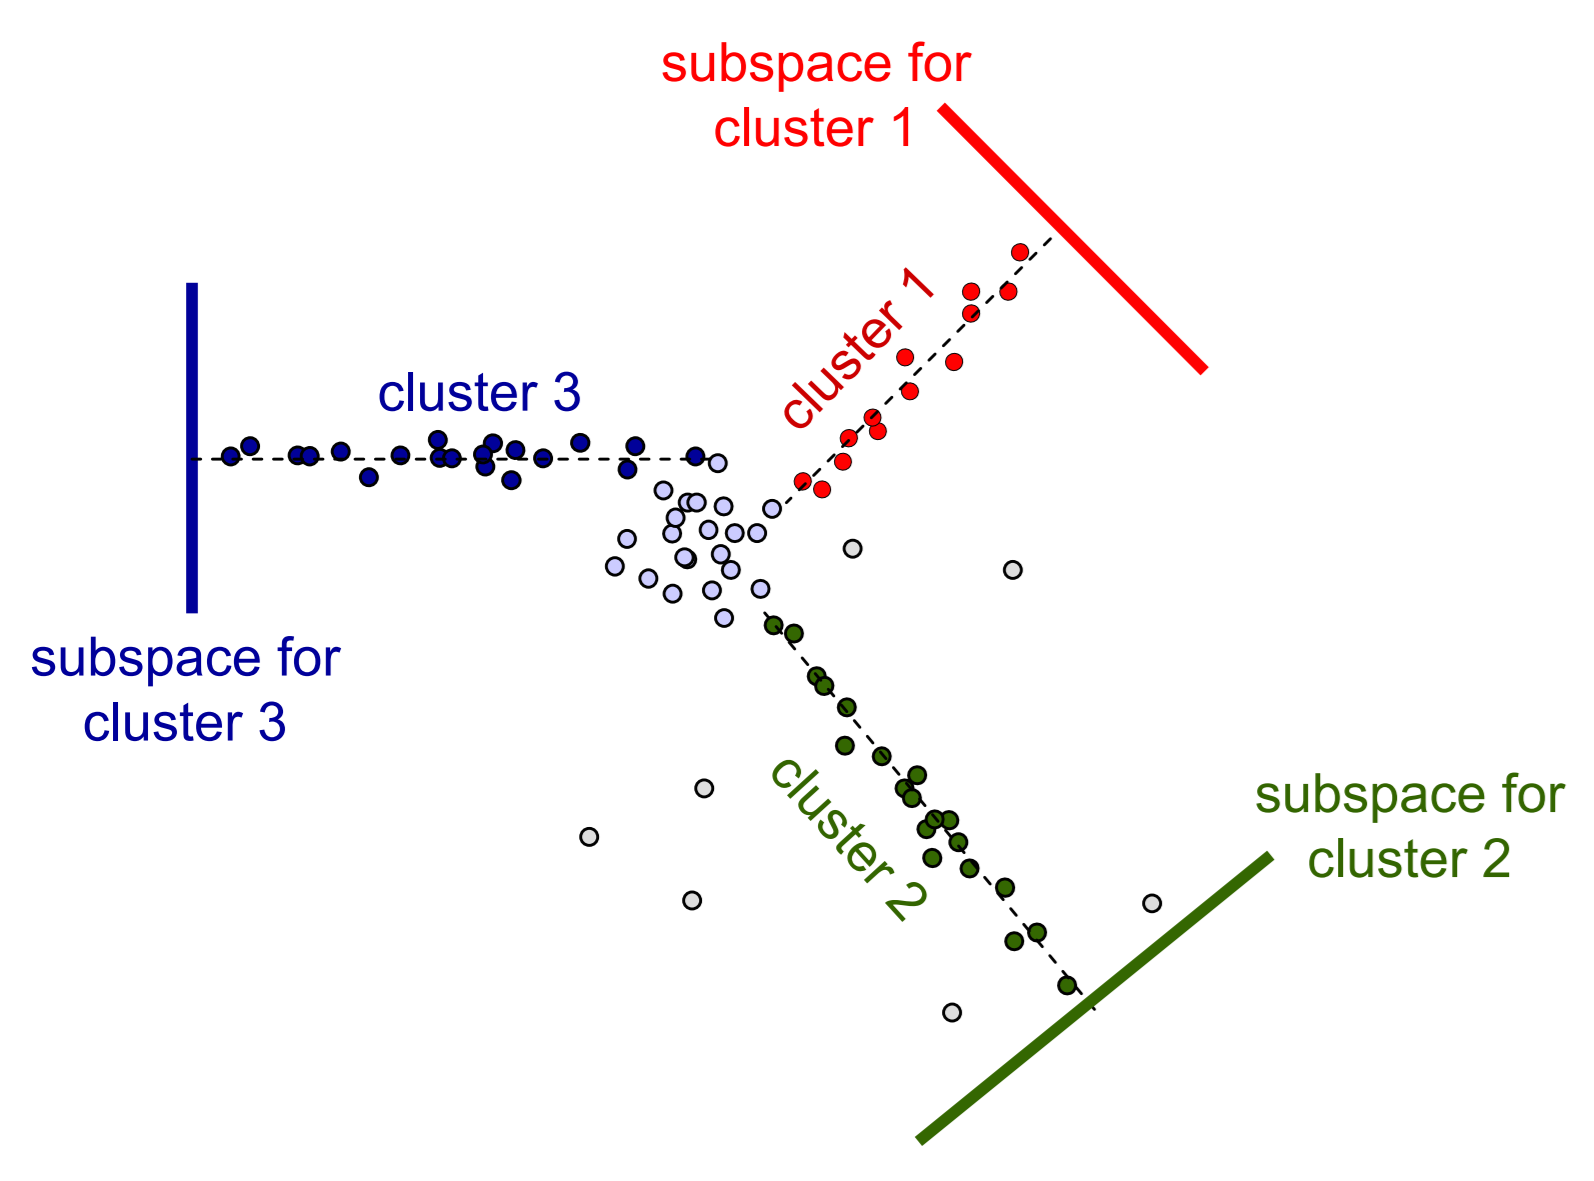
\includegraphics[width=0.6\textwidth]{figures/subcluex.png}
    \caption{Artificial example of arbitrarily oriented subspace clusters~\cite[Ch.3]{zimek2009correlation}.}
    \label{fig:corrclusex}
\end{figure}